\section{臨界と原子炉}

\subsection{中性子増倍率}
\label{subsec:multipilication_factor}
核分裂連鎖反応では、核分裂の反応数が指数関数的に増減する。
1つの中性子が核分裂を引き起こし、2つの中性子が放出される体系を考える。この2つの核分裂中性子がどちらも
次の核分裂を起こす場合、この体系の中性子増倍率$k$は次のようになる。
\begin{equation}
  k = \frac{\text{発生した核分裂中性子のうち核分裂を起こす数}}{\text{核分裂を起こした中性子数}} = \frac{2}{1} = 2
\end{equation}
実際には核分裂反応はバラバラなタイミングで起こるが、簡単のために「世代」という概念を導入して考える。
丁度アニメーションのフレームと同じで、バラバラなタイミングで起こる核分裂反応を、あるタイミングで一気に
発生するものとして考える。1フレームあたりの時間は、核分裂が発生してから次の核分裂が発生するまでの平均的な
時間を使う。この時間を\emph{即発中性子寿命}、または\emph{世代時間}と呼ぶ。
中性子増倍率はある世代の中性子数を一つ前の世代の中性子数で割ったものとしても定義される。
\begin{equation}
  \label{eq:multi_factor}
  k = \frac{\text{ある世代の中性子数}}{\text{一つ前の世代の中性子数}}
\end{equation}
この中性子増倍率$k$が1より大きい状態を\emph{超臨界}、1より小さい状態を\emph{未臨界}、1の状態を\emph{臨界}と呼ぶ。
\[
k \; \left\{
  \begin{array}{ll}
    > 1 & \text{超臨界} \\
    = 1 & \text{臨界} \\
    < 1 & \text{未臨界}
  \end{array}
\right.
\]

\subsection{中性子と原子核の反応}
中性子は電荷を持たないため原子核に近づきやすく、原子核と\SI{e-12}{\centi\metre}程度まで近づくと
原子核と相互作用する。この相互作用は、大きく散乱反応(scattering)と吸収反応(absorption)に分けられる。

\subsubsection{散乱反応}
散乱反応はさらに\emph{弾性散乱}(elastic scattering)と\emph{非弾性散乱}(inelastic scattering)の2つに分けられる。
弾性散乱では中性子と原子核の運動エネルギーは保存されるため、一般には中性子の運動エネルギーの一部が原子核(ターゲット核)
に移り中性子の運動方向とエネルギーが変化する。弾性散乱には、中性子が原子核に取り込まれずに原子核のポテンシャルで散乱される
ポテンシャル散乱と、中性子が一旦原子核に取り込まれ複合核となった後にエネルギーを失わずに放出される共鳴散乱がある。
非弾性散乱ではターゲット核に移ったエネルギーの一部が原子核の励起エネルギーに使われる。
そのため、非弾性散乱は中性子のエネルギーがターゲット核の最低の励起エネルギーよりも大きい場合にのみ起こる。
Fig.~\ref{fig:neutron_scattering}は、いくつかの核種の弾性散乱断面積を示している。黒鉛のように配列的に並ぶ材料に
対しては、低エネルギー中性子は回析を起こす(干渉性散乱)。また、水分子の水素原子のように、結合によって
自由に動き回れないことによる断面積の変化も見られる(非干渉性非弾性散乱)。
中エネルギー領域の中性子に対しては核力のポテンシャルによって散乱し、断面積は一定の値を示す。
高エネルギーの領域の中性子に対しては核力のポテンシャルを超えて原子核に取り込まれる部分が出てくる。

Fig.~\ref{fig:neutron_inelastic_scattering}は、\ce{^{238}U}と\ce{^{90}Zr}の非弾性散乱断面積、
Fig.~\ref{fig:neutron_inelastic_scattering_U238}は\ce{^{238}U}の励起準位を考慮した非弾性散乱断面積を示している。


\begin{figure}[htbp]
  \centering
  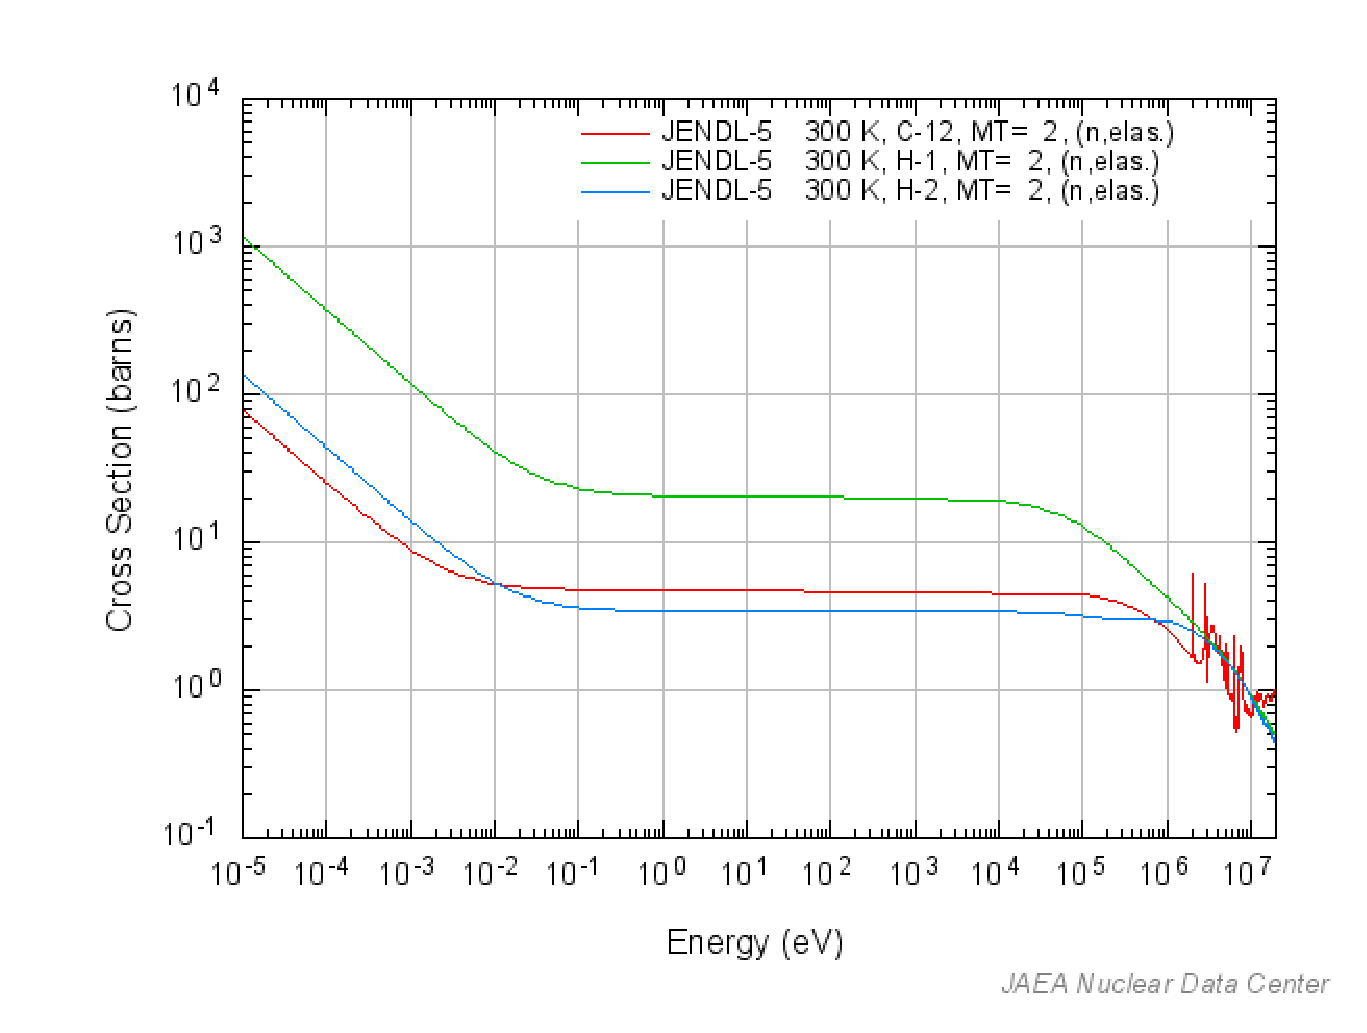
\includegraphics[width=0.8\textwidth]{figure/CrossSecElastic.eps}
  \caption{\ce{^{12}C},\ce{^{1}H},\ce{^{2}H}の弾性散乱(MT=2)の断面積}
  \label{fig:neutron_scattering}
\end{figure}

\begin{figure}[htbp]
  \centering
  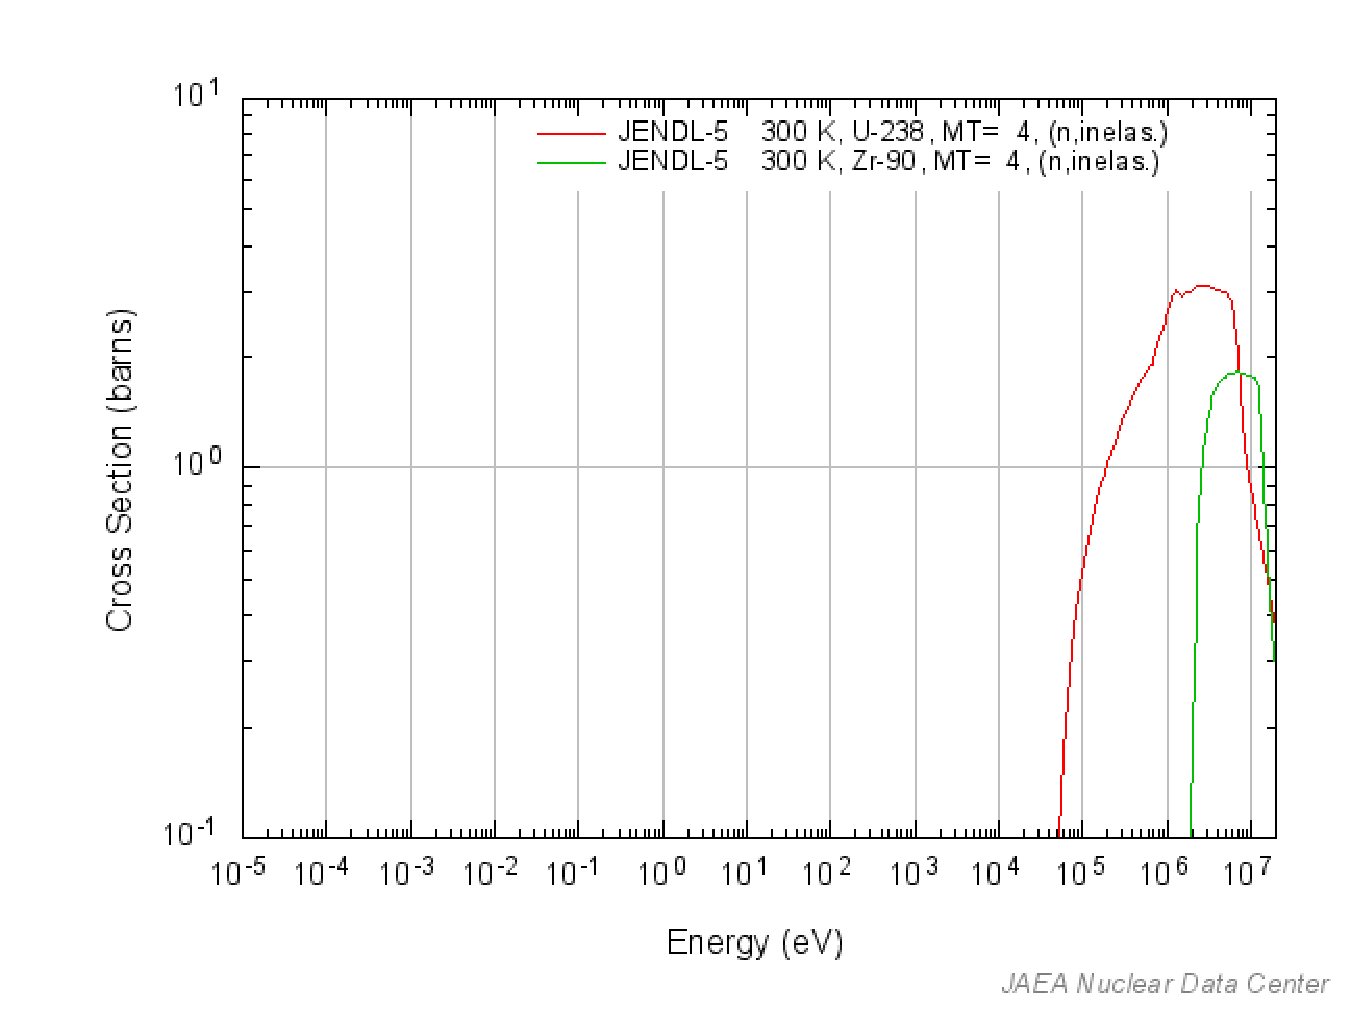
\includegraphics[width=0.8\textwidth]{figure/U238Zr90Inela.eps}
  \caption{\ce{^{238}U},\ce{^{90}Zr}の非弾性散乱(MT=4)の断面積}
  \label{fig:neutron_inelastic_scattering}
\end{figure}

\begin{figure}[htbp]
  \centering
  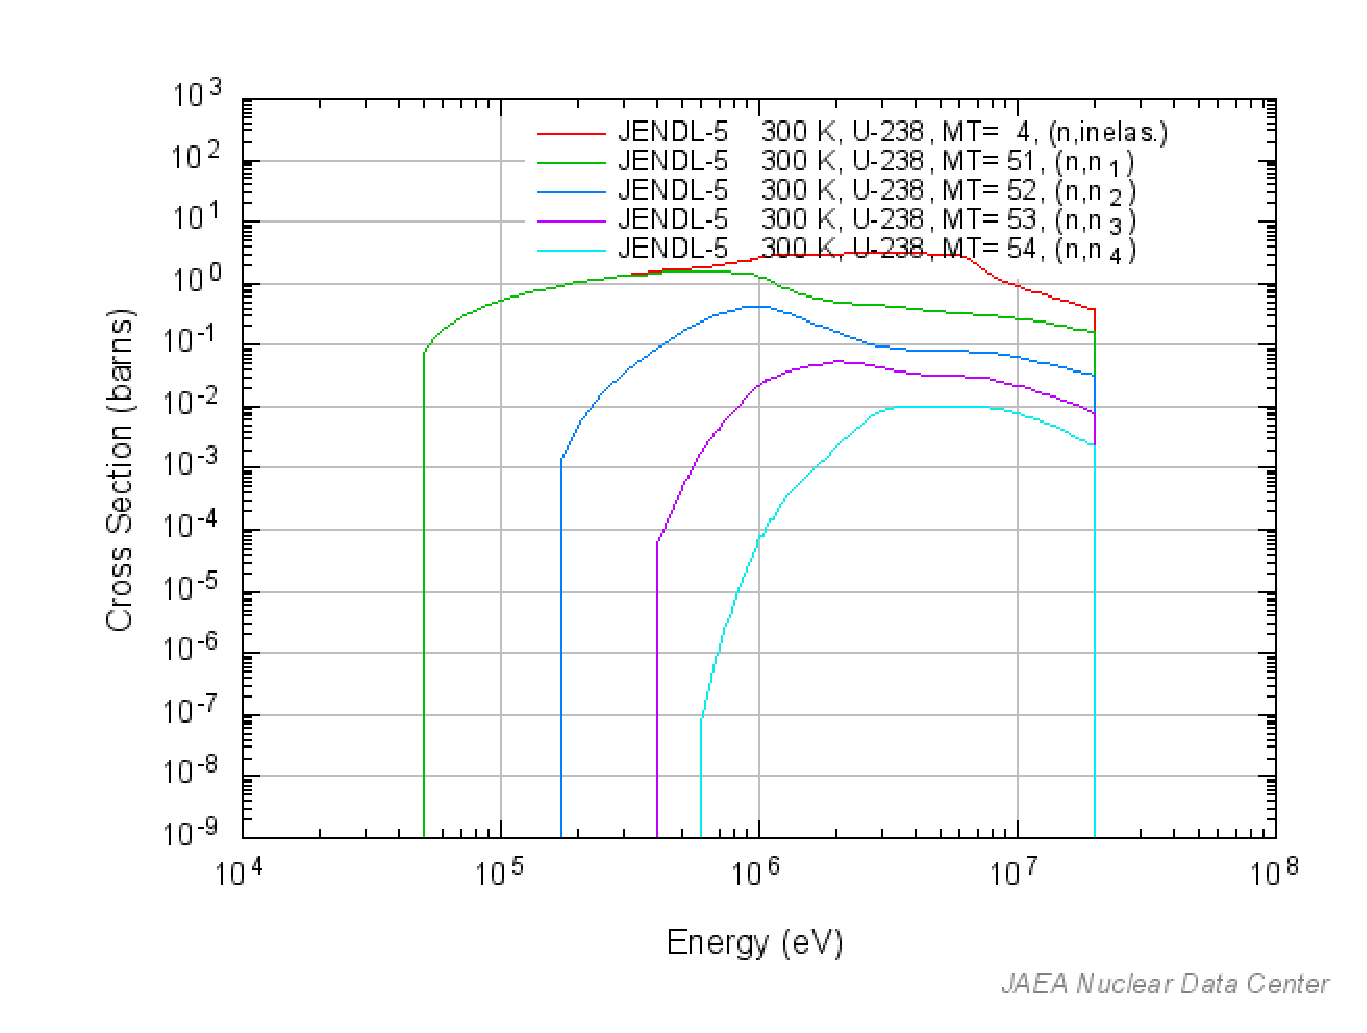
\includegraphics[width=0.8\textwidth]{figure/U238Inela_nx.eps}
  \caption{\ce{^{238}U}の非弾性散乱(MT=4,51,52,53,54)の断面積}
  \label{fig:neutron_inelastic_scattering_U238}
\end{figure}


\subsubsection{吸収反応}
原子核に中性子が取り込まれると、入射中性子のエネルギーと中性子の結合エネルギーの和の分だけ励起された複合核
が形成される。この複合核は不安定であるため、その後様々な反応を起こして安定な状態に戻ろうとする。
吸収反応この過程を経る反応の総称(散乱反応は除く)でその後の反応によってさらに多くの種類に分けられる。
これに分類されるものとしては、複合核から$\gamma$線を放出する放射捕獲反応、荷電粒子を放出する荷電粒子放出反応などがある。
原子炉において利用される核分裂反応や、入射中性子のエネルギーが高い場合に起こる2個以上の中性子が放出される反応も
この吸収反応に分類される。
Fig.~\ref{fig:neutron_absorption_Sm149}は、\ce{^{149}Sm}の(n,$\gamma$)反応、
Fig.~\ref{fig:neutron_capture_B10}は\ce{^{10}B}の(n,$\alpha$)反応、
Fig.~\ref{fig:neutron_fission}は\ce{^{235}U}の核分裂反応の断面積を示している。

それぞれの反応で共通して、低エネルギー領域では$1/v$に比例して断面積は減少している。
共鳴を持つ核種では中エネルギー領域で共鳴を起こすことも共通しているが、高エネルギー領域では捕獲断面積
は単調に減少するのに対し、核分裂断面積は階段状に増加することが分かる。
これは高エネルギーの中性子による核分裂反応では、中性子が吸収されてからすぐには割れず、1つ以上の中性子を
放出してから核分裂を起こす、マルチチャンス核分裂が存在するためである。
Fig.~\ref{fig:neutron_fission_U238}は、\ce{^{238}U}の核分裂反応において、分裂前に放出される
中性子の数ごとに分けた断面積(MT=19,20,21)と、すべての核分裂断面積の和(MT=18)を示している。

\begin{figure}[htbp]
  \centering
  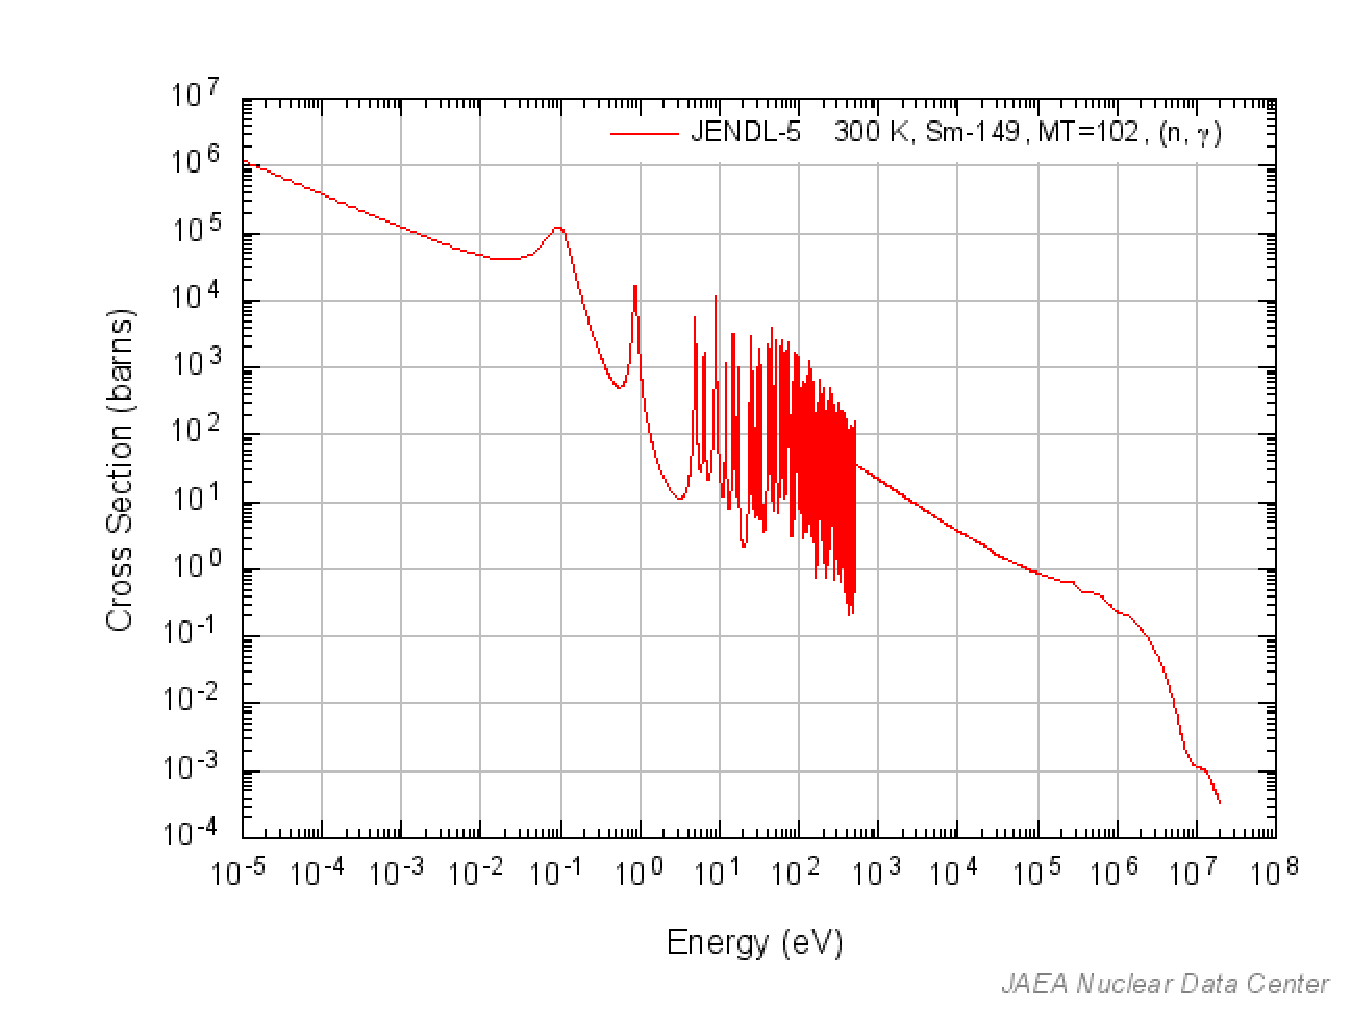
\includegraphics[width=0.8\textwidth]{figure/SmMT102.eps}
  \caption{\ce{^{149}Sm}の吸収反応(MT=102)の断面積}
  \label{fig:neutron_absorption_Sm149}
\end{figure}

\begin{figure}[htbp]
  \centering
  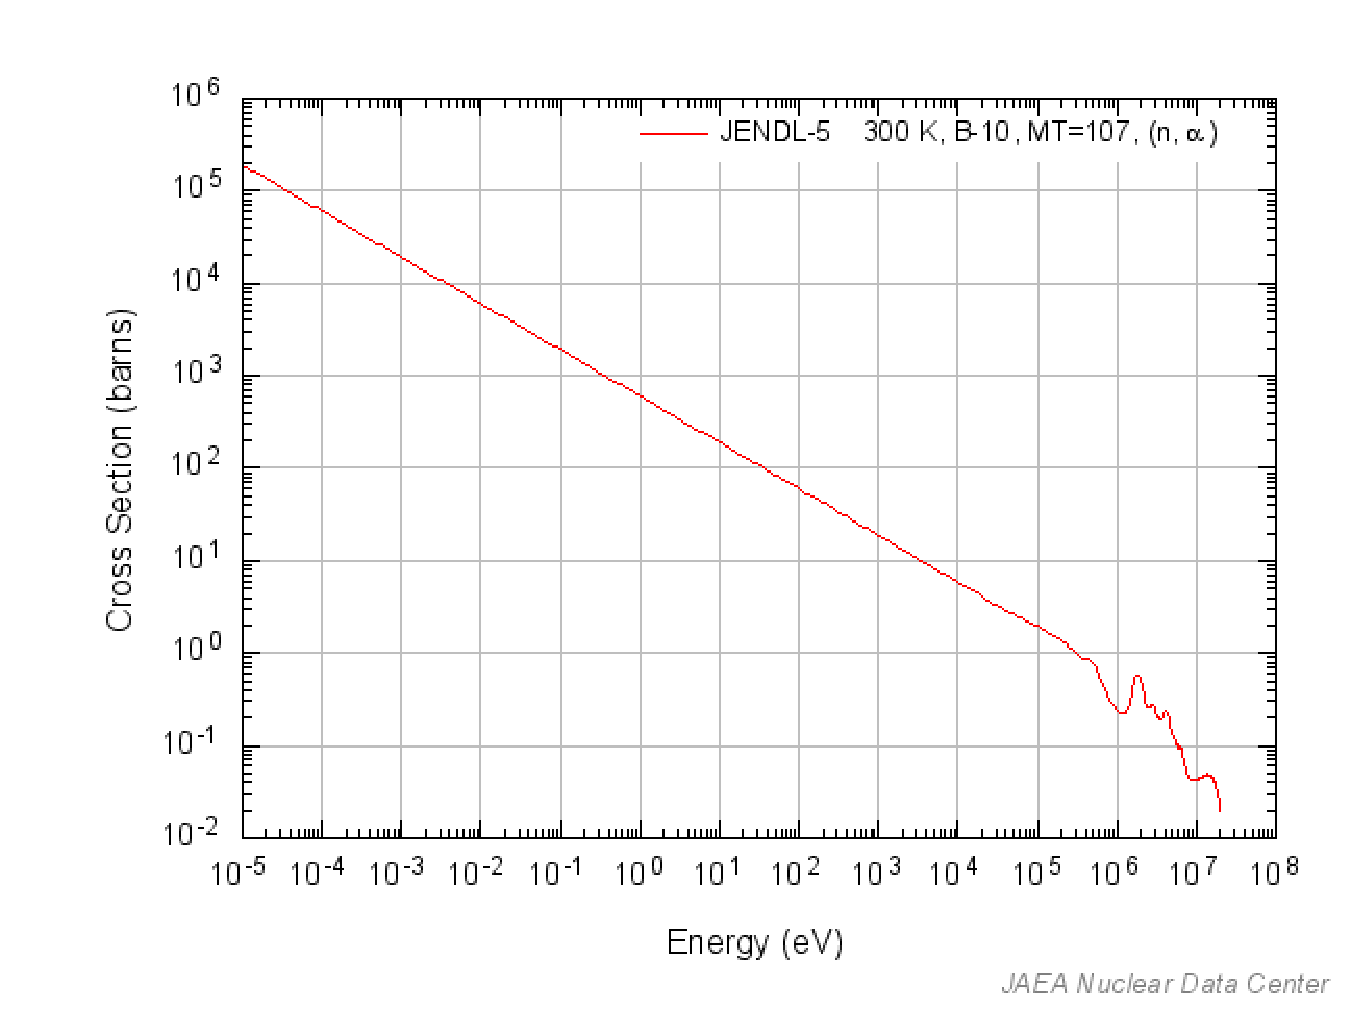
\includegraphics[width=0.8\textwidth]{figure/B10MT107.eps}
  \caption{\ce{^{10}B}の吸収反応(MT=107)の断面積}
  \label{fig:neutron_capture_B10}
\end{figure}

\begin{figure}[htbp]
  \centering
  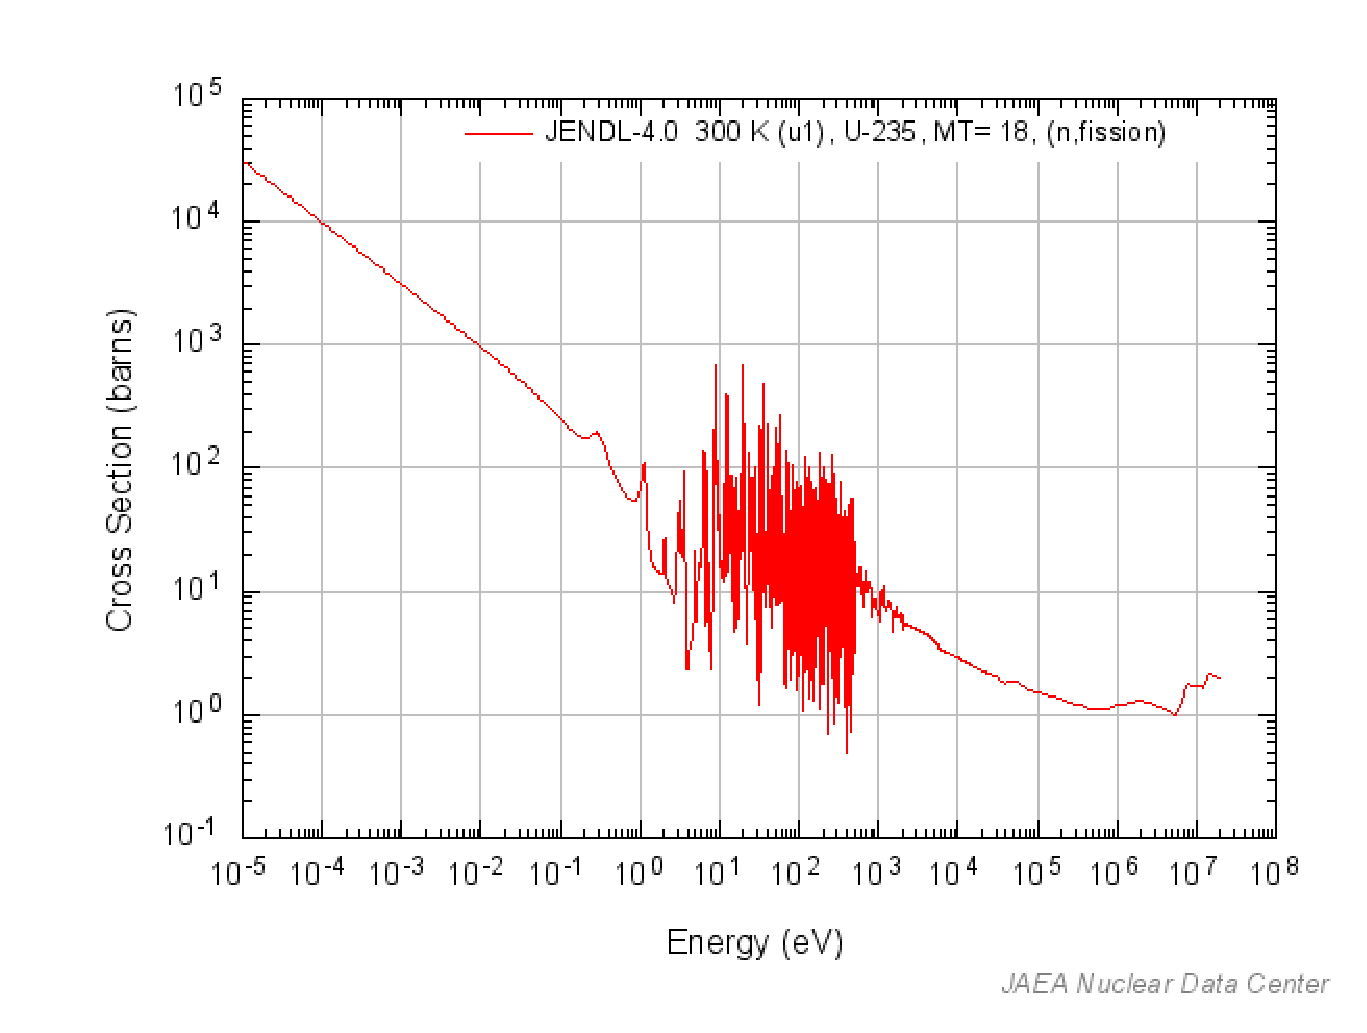
\includegraphics[width=0.8\textwidth]{figure/U235Fission.eps}
  \caption{\ce{^{235}U}の核分裂反応(MT=18)の断面積}
  \label{fig:neutron_fission}
\end{figure}

\begin{figure}[htbp]
  \centering
  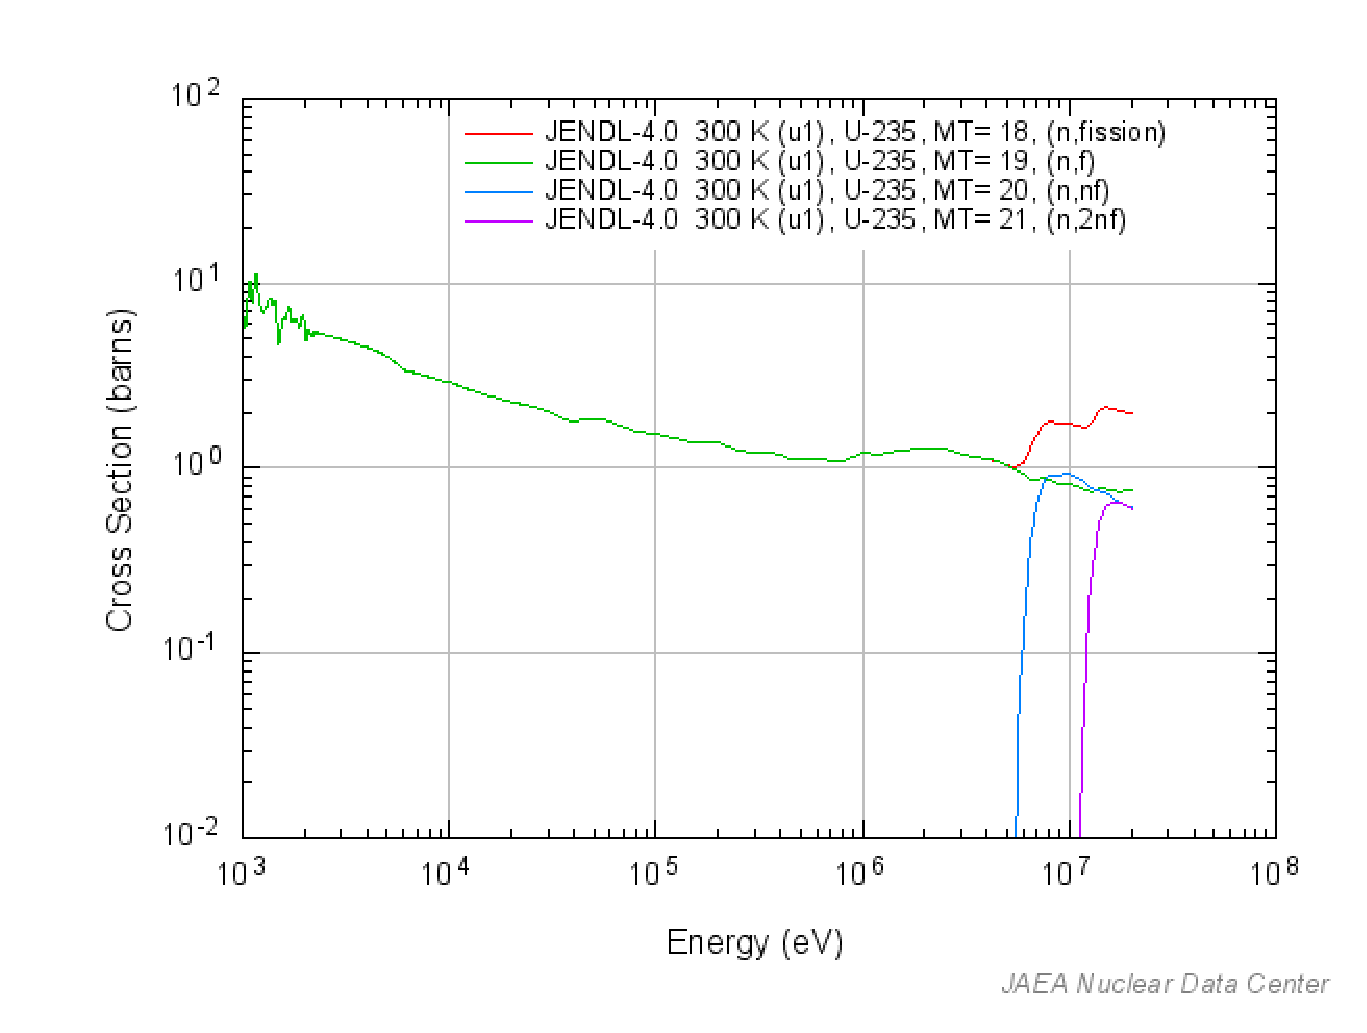
\includegraphics[width=0.8\textwidth]{figure/U235Fiss_xnf.eps}
  \caption{\ce{^{235}U}の核分裂反応(MT=18,19,20,21)の断面積}
  \label{fig:neutron_fission_U238}
\end{figure}

\clearpage

\subsection{臨界}
\ref{subsec:multipilication_factor}節で述べたように、臨界状態では中性子増倍率$k$は1で、
核分裂連鎖反応は外部から中性子を供給すること無しに、時間とともに増えも減りもせず一定の状態に維持される。
臨界を実現するための条件を調べるためにはFig.~\ref{fig:neutron_cycle}に示すような核分裂で発生した中性子の一生を考えることが適当である。

\begin{figure}[h]
  \centering
  \includegraphics[width=0.8\textwidth]{figure/neutron_cycle.eps}
  \caption{核分裂連鎖反応のサイクル}
  \label{fig:neutron_cycle}
\end{figure}

ある大きさの核分裂物質を含む体系を考える。
核分裂で発生したある世代の中性子は、体系から漏れるか、体系内にとどまるかのいずれかである。
体系にとどまる確率を$P_\text{NL}$とする。
体系にとどまった中性子は燃料に吸収されるか、燃料以外の物質に吸収されるかのいずれかである。
吸収されるとした場合に燃料に吸収される確率を$P_\text{aF}$とする。
燃料に吸収されたあと、それが捕獲反応ではなく核分裂反応を起こす確率を$P_\text{f}$とする。
核分裂を起こすと中性子を$\nu$個放出し、以下この過程を繰り返す。
\ref{eq:multi_factor}式より、増倍率$k$は次のように表される。
\begin{equation}
  k = P_\text{NL} \cdot P_\text{aF} \cdot P_\text{f} \cdot \nu
\end{equation}
以下この式をさらに定量的に考える。

\subsubsection{熱中性子利用率}
まず中性子が吸収される場合に、燃料に吸収される確率$P_\text{aF}$を考える。
燃料に吸収される確率は、燃料の中性子吸収断面積$\Sigma_\text{a}^{F}$と、
体系全体の中性子吸収断面積$\Sigma_\text{a}$の比で表される。
\begin{equation}
  P_\text{aF} = \frac{\Sigma_\text{a}^{F}}{\Sigma_\text{a}}
\end{equation}

この量を\emph{熱中性子利用率}(thermal utilization factor)と呼び$f$という記号で表す。
\begin{equation}
  f = P_\text{aF} = \frac{\Sigma_\text{a}^{F}}{\Sigma_\text{a}}
\end{equation}

\subsubsection{$\eta$(イータ)}
次に、燃料に吸収された中性子が核分裂を起こす確率$P_\text{f}$を考える。
$P_\text{f}$は燃料に吸収されたときに核分裂を起こす確率であるから、
燃料の核分裂断面積$\Sigma_\text{f}^{F}$と燃料の中性子吸収断面積$\Sigma_\text{a}^{F}$の比で表される。
\begin{equation}
  P_\text{f} = \frac{\Sigma_\text{f}^{F}}{\Sigma_\text{a}^{F}}= \frac{\sigma_\text{f}^{F}}{\sigma_\text{a}^{F}}
\end{equation}

核分裂を起こすと平均して$\nu$個の中性子が放出されるので、核燃料により中性子が再生される割合を
記号$\eta$で次のように表す。
\begin{equation}
  \eta = \nu \cdot \frac{\sigma_\text{f}^{F}}{\sigma_\text{a}^{F}} = \nu P_\text{f}
\end{equation}

この値を\emph{再生率}(reproduction factor)と呼ぶ。

\subsubsection{無限増倍率}
以上の値を用いて、増倍率$k$を書き直すと次のようになる。
\begin{equation}
  k = P_\text{NL} \cdot f \cdot \eta
\end{equation}

$P_\text{NL}$は体系の形に依存するため考えるのが難しい。そこで無限に大きい原子炉を考えて$P_\text{NL}$を1とする。
この時の増倍率を\emph{無限増倍率}(infinite multiplication factor)と呼び、記号$k_\infty$で表す。
\begin{equation}
  k_\infty = f \cdot \eta
\end{equation}

実際には$P_\text{NL}$は1より小さいため、$k_\infty > 1$でない限り原子炉が臨界になることは無い。

\subsubsection{高速中性子核分裂因子}
以上の式では、熱中性子による核分裂のみが考えられているが、
原子炉では高速中性子による核分裂も利用される。これはその世代の中性子の数をすこし増やす。
この硬化を表す量を高速中性子核分裂因子(fast fission factor)と呼び、記号$\epsilon$で表す。
\begin{equation}
  \epsilon = \frac{\text{高速および熱中性子による全核分裂中性子数}}{\text{熱中性子による核分裂中性子数}}
\end{equation}

\subsubsection{共鳴を逃れる確率}
また、中性子が発生直後の高速領域から熱領域まで減速する過程で、\ce{^{238}U}のような
共鳴を持つ核種に吸収されて失われることも考慮する必要がある。
減速過程で吸収されずに熱中性子領域まで減速される中性子の割合を\emph{共鳴を逃れる確率}(resonance escape probability)と呼び、
記号$p$で表す。

この量は燃料と減速材の割合に大きく依存するとともに、その形状、配列にも依存する。

\subsubsection{4因子公式と6因子公式}
以上の値を用いて増倍率$k$を表すと、次のようになる。
\begin{equation}
  k_\infty = \epsilon \cdot p \cdot \eta \cdot f
\end{equation}

この無限増倍率を表す式を\emph{4因子公式}と呼ぶ。
さらに中性子が体系から漏れない確率$P_\text{NL}$を、高速中性子の漏れない確率$P_\text{FNL}$
と熱中性子の漏れない確率$P_\text{TNL}$に分けると増倍率の式は次のように書き直せる。
\begin{equation}
  k = k_\infty P_\text{NL} =\epsilon \cdot p \cdot \eta \cdot f
\cdot P_\text{FNL} \cdot P_\text{TNL}
\end{equation}

この式を\emph{6因子公式}と呼び、この$k$を\emph{実効増倍率}(effective multiplication factor)と呼ぶ。

\subsection{代表的な原子炉}
ここでは、加圧水型原子炉(PWR)、沸騰水型原子炉(BWR)、高速炉の3つの原子炉を紹介する。
\subsubsection{加圧水型原子炉(PWR)}
加圧水型原子炉(Pressurized Water Reactor: PWR)は、一次冷却材兼減速材として
軽水を用い、燃料として低濃縮二酸化ウラン(\ce{UO_2})を用いる原子炉であり、主として熱中性子によって核分裂が発生する。
PWRでは、一次冷却材が高圧(約15MPa)に保たれた状態で炉心下部から流入し、炉心上部から出ていき、
蒸気発生器において二次冷却材を沸騰させる。
高圧により冷却材の沸騰が起こらないため、この間の冷却材の密度変化は、水密度が炉心内で70\%以上も変化するBWRに比べるとはるかに小さい。
水密度は中性子の減速を通じて炉内の核分裂の増減に影響を与えるが、冷却材密度の変化の小さいPWR炉心内の
中性子エネルギースペクトルの空間的変化はBWRに比べて小さく、均質に近い炉心構成となることが特徴である。
また、運転中の反応度制御を冷却材中に溶かしたホウ素により行うことも特徴である、そのため、PWRでは
運転時において制御棒はほとんど全引き抜き状態である。制御棒を挿入するとその近辺の出力分布にひずみが生じる
が、PWRでは炉心全体にまんべんなく存在する冷却材中のホウ素によって出力を制御するため、反応度制御の観点からも
BWR炉心に比べて核的に均一な炉心構造であるといえる。

\subsubsection{沸騰水型原子炉(BWR)}
沸騰水型原子炉(BWR: Boiling Water Reactor)は、PWRと同じく一次冷却材兼減速材として軽水を用い、燃料として
低濃縮二酸化ウラン(\ce{UO_2})を用いる原子炉であり、主として熱中性子によって核分裂が発生する。

BWRでは、炉心内で冷却材が沸騰し、蒸気泡(ボイド:Void)が発生する。炉心内のボイドは炉心中の軽水の密度を
大きく変化させるため、BWRでは炉心内の中性子エネルギースペクトルが空間的に変化しやすい。
冷却材は再循環ポンプによって駆動され、炉心下部から炉心に流入した後、燃料棒にそって上昇し
燃料からの熱をうけて沸点に到達し、一部はボイドとなる。BWR炉心における
平均ボイド率は約40\%であり、炉心出口では約70\%に達する。BWRの運転圧力は約7MPaであり、PWRの半分程度である。
BWRの特徴として、ボイド反応度が挙げられる。
ボイド反応度とは、炉心内のボイド率が変化したときに生じる反応度の変化であり、BWRでは負の反応度係数を持つ。
出力が上昇し、ボイド率が増加すると、冷却材の密度が減少し、減速材の効果が低下するため、熱中性子の数が減少し、
核分裂反応が減少する。これがBWRに固有の安全性を与えるとともに、再循環流量の調整による出力の制御を可能にしている。
\subsubsection{高速炉}
高速炉の目的は、エネルギーの生産と同時に核燃料の生成も行い、核燃料の資源を有効に利用することである。

上記の軽水炉において、熱中性子によって核分裂をおこすのは天然ウランの内約0.7\%を占める\ce{^{235}U}のみであるが、
中性子を\ce{^{238}U}に吸収させると、熱中性子で核分裂を起こす\ce{^{239}Pu}が生成される。
前節で述べたように1個の中性子が燃料に吸収されると、$\eta$個の中性子が再生される。
そのうちの1個は核分裂連鎖反応を維持するために必要な中性子であるので、残りの$\eta - 1$個を\ce{^{238}U}や\ce{^{232}Th}
といった物質に吸収させることで、核燃料を生成し、核燃料の資源を飛躍的に増やすことが期待できる。
$\eta$の値が2を超えると、1個の中性子で2個以上の中性子が再生されることになり、核燃料の\emph{増殖}が可能になる。
熱中性子に対する$\eta$の値は\ce{^{235}U}や\ce{^{239}Pu}ではわずかに2を超える程度であり、中性子の漏れや
他の物質への吸収を考慮すると、熱中性子炉では核燃料の増殖は難しい。
しかし、中性子のエネルギーが100keV以上の領域では$\eta$の値はエネルギーとともに急激に大きくなり、
$\eta > 2$つまり、燃料の増殖を実現出来る可能性が高く、この傾向は特に\ce{^239Pu}に顕著である。

高速炉では、中性子を減速させずに核分裂連鎖反応を維持する必要があるため、冷却には軽水以外の媒体を用いる必要があるため、
冷却材としてはナトリウムや鉛ビスマス、\ce{He}ガスなどが用いられる。
また、高速領域での核分裂断面積は熱中性子に対するものよりも2~3桁小さくなるため、炉心出力を軽水炉並みにするために
中性子束を大きくすること、また\ce{Pu}の重量割合を大きくする必要がある。

% 章ごとの参考文献欄
\printbibliography[segment=\therefsegment,heading=subbibliography]

\newpage
